\documentclass[12pt,a4paper]{article}

% ─── Packages ───────────────────────────────────────────────────
\usepackage[margin=1in]{geometry}
\usepackage{amsmath,amssymb,amsthm,mathtools}
\usepackage{hyperref}
\usepackage{cleveref}
\usepackage{tikz-cd}
\usepackage{tikz}
\usetikzlibrary{positioning,arrows.meta,decorations.markings,calc,shapes,backgrounds}
\usepackage{enumitem}
\usepackage{xcolor}
\usepackage{fancyhdr}
\usepackage{everypage}
\usepackage{abstract}
\usepackage{booktabs}
\usepackage{float}
\usepackage{listings}

% ─── GrokRxiv DOI Sidebar ──────────────────────────────────────
\definecolor{grokgray}{RGB}{110,110,110}
\AddEverypageHook{%
  \ifnum\value{page}=1
    \begin{tikzpicture}[remember picture, overlay]
      \node[rotate=90, anchor=south, font=\Large\sffamily\bfseries\color{grokgray}, inner sep=0pt]
      at ([xshift=38pt, yshift=0.52\paperheight]current page.south west)
      {GrokRxiv:2026.03.developmental-programs-orchestration\quad [\,bio.PL\,]\quad 31 Mar 2026};
    \end{tikzpicture}
  \fi
}

% ─── Theorem Environments ──────────────────────────────────────
\newtheorem{theorem}{Theorem}[section]
\newtheorem{lemma}[theorem]{Lemma}
\newtheorem{proposition}[theorem]{Proposition}
\newtheorem{corollary}[theorem]{Corollary}
\newtheorem{definition}[theorem]{Definition}
\newtheorem{example}[theorem]{Example}
\newtheorem{remark}[theorem]{Remark}
\newtheorem{axiom}[theorem]{Axiom}
\newtheorem{conjecture}[theorem]{Conjecture}

% ─── Listings ──────────────────────────────────────────────────
\definecolor{codegreen}{RGB}{40,140,40}
\definecolor{codegray}{RGB}{100,100,100}
\definecolor{codepurple}{RGB}{120,50,160}
\definecolor{backcolour}{RGB}{248,248,248}
\lstdefinestyle{haskellstyle}{
    backgroundcolor=\color{backcolour},
    commentstyle=\color{codegreen}\itshape,
    keywordstyle=\color{codepurple}\bfseries,
    numberstyle=\tiny\color{codegray},
    stringstyle=\color{red!60!black},
    basicstyle=\ttfamily\small,
    breakatwhitespace=false,
    breaklines=true,
    captionpos=b,
    keepspaces=true,
    numbers=left,
    numbersep=5pt,
    showspaces=false,
    showstringspaces=false,
    showtabs=false,
    tabsize=2,
    language=Haskell,
    morekeywords={data,type,class,instance,where,deriving,newtype,module,import,qualified,as,do,let,in,case,of,if,then,else,forall}
}
\lstset{style=haskellstyle}

% ─── Custom Commands ───────────────────────────────────────────
\newcommand{\ie}{\textit{i.e.}}
\newcommand{\eg}{\textit{e.g.}}
\newcommand{\cf}{\textit{cf.}}
\newcommand{\Prog}{\texttt{Program}}
\newcommand{\Hox}{\texttt{Hox}}
\newcommand{\CellT}{\texttt{Cell}}
\newcommand{\StemCell}{\texttt{StemCell}}
\newcommand{\TermCell}{\texttt{TerminalCell}}
\newcommand{\Morphogen}{\texttt{Morphogen}}

% ─── Header / Footer ──────────────────────────────────────────
\pagestyle{fancy}
\fancyhf{}
\fancyhead[L]{\small Developmental Programs as Orchestration}
\fancyhead[R]{\small Paper 7 of 7 --- DNA-Lang}
\fancyfoot[C]{\thepage}
\renewcommand{\headrulewidth}{0.4pt}

% ─── Title ─────────────────────────────────────────────────────
\title{%
  \textbf{Developmental Programs as Orchestration:}\\[6pt]
  \Large A Type-Theoretic Framework for Morphogenesis\\[12pt]
  \large Paper 7 of 7 --- The DNA-Lang Project
}
\author{
  Matthew Long\\
  \textit{The YonedaAI Collaboration}\\
  Chicago, IL\\
  \texttt{matt@yoneda.ai}
}
\date{March 31, 2026}

\begin{document}
\maketitle

% ─── Abstract ──────────────────────────────────────────────────
\begin{abstract}
\noindent
We present a type-theoretic framework in which the developmental program
of a multicellular organism is modeled as a typed orchestration system.
Hox genes are formalized as the main module of a body-plan specification
language; morphogen gradients are cast as distributed, spatially-dependent
configuration; and cell-fate determination is expressed as progressive
type refinement from stem cells to terminally differentiated cells.
We introduce the \texttt{Program\textless{}OrganismDevelopment\textgreater{}}
type, whose inhabitants encode regulatory cascades as typed boot sequences,
apoptosis as graceful shutdown, and stem-cell self-renewal as an abstract
factory pattern with polymorphic constructors.  The Waddington landscape
is reinterpreted as a refinement-type lattice, morphogen gradients as
dependent types, Hox collinearity as a monotone functor, and organogenesis
as container orchestration.  A complete Haskell implementation is provided
that demonstrates the framework compiles and executes, bridging the gap
between developmental biology and programming-language theory.
\end{abstract}

\vspace{1em}
\noindent\textbf{Keywords:} developmental biology, type theory, Hox genes,
morphogenesis, Waddington landscape, dependent types, refinement types,
category theory, orchestration, DNA-Lang

\tableofcontents
\newpage

% ═══════════════════════════════════════════════════════════════
\section{Introduction: From Genome to Organism}\label{sec:intro}
% ═══════════════════════════════════════════════════════════════

The central mystery of developmental biology is how a single fertilized egg
gives rise to a complex multicellular organism with hundreds of distinct cell
types, intricate tissue architectures, and precisely patterned organ systems.
The genome, viewed as a static string over a four-letter alphabet, must be
\emph{executed} to produce a dynamic, three-dimensional living system.

This is, fundamentally, a \emph{programming problem}.

\begin{definition}[The Developmental Programming Problem]\label{def:dev-problem}
Given a genome $G$ over alphabet $\Sigma = \{A,T,C,G\}$ and an initial
cell state $c_0$, the developmental programming problem asks for the
existence of an execution semantics $[\![ - ]\!]$ such that
\[
  [\![ G ]\!](c_0) = \mathcal{O}
\]
where $\mathcal{O}$ is a well-formed organism satisfying the species-specific
body plan constraints $\Phi$.
\end{definition}

In classical computer science, orchestration refers to the automated
coordination of multiple services, containers, or processes to achieve
a complex workflow.  The analogy to development is striking:

\begin{itemize}[leftmargin=2em]
  \item \textbf{Genome $\leftrightarrow$ Source code}: The DNA sequence
    encodes the full specification.
  \item \textbf{Transcription factors $\leftrightarrow$ Schedulers}: Regulatory
    proteins decide which genes execute, when, and where.
  \item \textbf{Morphogen gradients $\leftrightarrow$ Configuration management}:
    Spatially varying signals configure cell behavior.
  \item \textbf{Cell fate $\leftrightarrow$ Type refinement}: As cells
    differentiate, their behavioral interface narrows.
  \item \textbf{Apoptosis $\leftrightarrow$ Graceful shutdown}: Programmed
    cell death removes unnecessary processes.
  \item \textbf{Stem cells $\leftrightarrow$ Factory patterns}: Self-renewing
    cells produce typed progeny on demand.
\end{itemize}

The DNA-Lang project has, through its preceding six papers, developed a
type-theoretic interpretation of genomic elements: coding sequences as
executable functions, regulatory sequences as control flow, noncoding RNA
as type-level metaprogramming, epigenetic marks as compiler pragmas,
repetitive elements as memory architecture, and structural DNA as the
runtime environment.  In this seventh and final paper, we synthesize
these perspectives into a unified account of \emph{developmental programs
as typed orchestration}.

\subsection{Contributions}

\begin{enumerate}[leftmargin=2em]
  \item A formal type \texttt{Program\textless{}OrganismDevelopment\textgreater{}}
    that captures the full developmental pipeline.
  \item Hox gene collinearity as a monotone functor between ordered sets.
  \item Morphogen gradients as spatially-dependent types.
  \item Cell-fate determination as refinement-type narrowing over the
    Waddington landscape.
  \item Regulatory cascades as typed boot sequences with dependency resolution.
  \item Apoptosis as graceful shutdown with resource cleanup.
  \item Stem cells as abstract factories with polymorphic constructors.
  \item Organogenesis as container orchestration.
  \item A complete, compiling Haskell implementation.
\end{enumerate}

\subsection{Organization}

\Cref{sec:hox} introduces Hox genes as the main module.
\Cref{sec:morphogens} formalizes morphogen gradients as distributed
configuration.  \Cref{sec:cellfate} presents cell-fate determination
as type refinement.  \Cref{sec:program-type} defines the core
\Prog{} type.  \Cref{sec:regulatory} treats regulatory cascades as
boot sequences.  \Cref{sec:apoptosis} models apoptosis as graceful
shutdown.  \Cref{sec:stemcells} casts stem cells as factory patterns.
\Cref{sec:waddington} reinterprets the Waddington landscape via
refinement types.  \Cref{sec:morphogen-dependent} introduces morphogen
gradients as dependent types.  \Cref{sec:hox-functor} establishes
Hox collinearity as a monotone functor.  \Cref{sec:organogenesis}
models organogenesis as container orchestration.
\Cref{sec:implementation} presents the Haskell implementation.
\Cref{sec:discussion} discusses implications and concludes.


% ═══════════════════════════════════════════════════════════════
\section{Hox Genes as the Main Module}\label{sec:hox}
% ═══════════════════════════════════════════════════════════════

Hox genes encode homeodomain transcription factors that specify segment
identity along the anterior--posterior (A--P) axis.  In virtually all
bilaterian animals, Hox genes are organized in genomic clusters, and
their expression exhibits \emph{collinearity}: genes located 3$'$ in
the cluster are expressed more anteriorly and earlier in development
than genes located 5$'$.

\begin{definition}[Hox Cluster]\label{def:hox-cluster}
A \emph{Hox cluster} is a finite ordered set
$\mathcal{H} = (H_1, H_2, \ldots, H_n)$ of Hox genes equipped with:
\begin{enumerate}
  \item A \emph{chromosomal order} $\leq_{\text{chr}}$ reflecting
    physical position on the chromosome.
  \item A \emph{spatial expression function}
    $\sigma : \mathcal{H} \to \mathcal{P}(\text{A--P axis})$ mapping
    each gene to the set of body segments where it is expressed.
  \item A \emph{temporal expression function}
    $\tau : \mathcal{H} \to \mathbb{R}_{\geq 0}$ mapping each gene
    to its activation time.
\end{enumerate}
\end{definition}

\begin{axiom}[Spatial Collinearity]\label{ax:spatial-col}
For Hox genes $H_i, H_j$ with $i \leq_{\text{chr}} j$, we have
\[
  \max(\sigma(H_i)) \leq \max(\sigma(H_j))
\]
That is, chromosomally later genes are expressed in more posterior
segments.
\end{axiom}

\begin{axiom}[Temporal Collinearity]\label{ax:temporal-col}
For Hox genes $H_i, H_j$ with $i \leq_{\text{chr}} j$, we have
$\tau(H_i) \leq \tau(H_j)$.
That is, chromosomally earlier genes are activated earlier in
development.
\end{axiom}

In programming-language terms, the Hox cluster functions as the
\texttt{main} module of the developmental program: it is the
entry point that establishes the high-level body plan before
delegating to subordinate modules for organ-specific differentiation.

\begin{proposition}[Hox Cluster as Main Module]\label{prop:hox-main}
The Hox cluster $\mathcal{H}$ acts as a main module in the sense
that:
\begin{enumerate}
  \item It is activated early in development (boot priority).
  \item It establishes the global coordinate system (A--P axis).
  \item Downstream modules (organ-specific gene networks) depend
    on Hox-established segment identity.
  \item Mutations in $\mathcal{H}$ produce \emph{homeotic
    transformations}---global structural errors analogous to
    type errors in the main module.
\end{enumerate}
\end{proposition}

The Hox code is ``read'' by downstream regulatory networks, which
interpret segment identity as a type tag determining which
developmental subroutines to execute in each segment.

\begin{figure}[H]
\centering
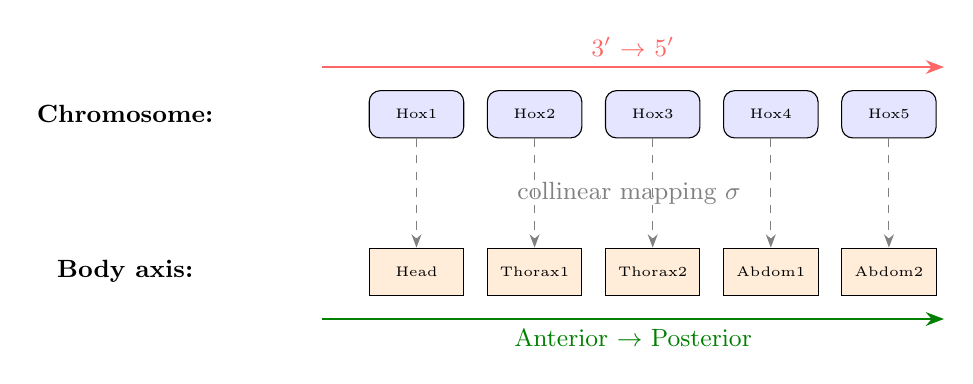
\begin{tikzpicture}[
  gene/.style={draw, rounded corners, minimum width=1.2cm, minimum height=0.6cm, fill=blue!10},
  segment/.style={draw, minimum width=1.2cm, minimum height=0.6cm, fill=orange!15},
  >=Stealth
]
  % Chromosome
  \node[font=\small\bfseries] at (-2.2, 2) {Chromosome:};
  \foreach \i/\name in {1/Hox1, 2/Hox2, 3/Hox3, 4/Hox4, 5/Hox5} {
    \node[gene] (g\i) at (\i*1.5, 2) {\tiny \name};
  }
  \draw[->, thick, red!60] (0.3, 2.6) -- (8.2, 2.6) node[midway, above, font=\small] {3$'$ $\to$ 5$'$};

  % Body segments
  \node[font=\small\bfseries] at (-2.2, 0) {Body axis:};
  \foreach \i/\name in {1/Head, 2/Thorax1, 3/Thorax2, 4/Abdom1, 5/Abdom2} {
    \node[segment] (s\i) at (\i*1.5, 0) {\tiny \name};
  }
  \draw[->, thick, green!50!black] (0.3, -0.6) -- (8.2, -0.6) node[midway, below, font=\small] {Anterior $\to$ Posterior};

  % Mapping arrows
  \foreach \i in {1,...,5} {
    \draw[->, dashed, gray] (g\i) -- (s\i);
  }

  \node[font=\small, text=gray] at (4.2, 1) {collinear mapping $\sigma$};
\end{tikzpicture}
\caption{Spatial collinearity: chromosomal order maps to body-axis position.}
\label{fig:collinearity}
\end{figure}


% ═══════════════════════════════════════════════════════════════
\section{Morphogen Gradients as Distributed Configuration}\label{sec:morphogens}
% ═══════════════════════════════════════════════════════════════

Morphogens are signaling molecules secreted by localized source cells
that form concentration gradients across developing tissues.  Cells
respond to the local morphogen concentration by activating different
gene-expression programs, effectively receiving \emph{positional
information} encoded in a continuous chemical signal.

\begin{definition}[Morphogen Field]\label{def:morphogen-field}
A \emph{morphogen field} is a triple $(M, \Omega, c)$ where:
\begin{itemize}
  \item $M$ is the morphogen identity (\eg, Sonic Hedgehog, Wnt, BMP).
  \item $\Omega \subseteq \mathbb{R}^3$ is the tissue domain.
  \item $c : \Omega \times \mathbb{R}_{\geq 0} \to \mathbb{R}_{\geq 0}$
    is the concentration function, where $c(\mathbf{x}, t)$ gives the
    morphogen concentration at position $\mathbf{x}$ and time $t$.
\end{itemize}
\end{definition}

The \emph{French flag model} (Wolpert, 1969) partitions the tissue
domain into discrete fate zones based on concentration thresholds:

\begin{definition}[French Flag Partition]\label{def:french-flag}
Given a morphogen field $(M, \Omega, c)$ and threshold concentrations
$\theta_1 > \theta_2 > \cdots > \theta_{k-1} > 0$, the \emph{French
flag partition} at time $t$ is
\[
  \Omega = \Omega_1(t) \sqcup \Omega_2(t) \sqcup \cdots \sqcup \Omega_k(t)
\]
where $\Omega_i(t) = \{ \mathbf{x} \in \Omega \mid \theta_{i-1} \geq
c(\mathbf{x},t) > \theta_i \}$ (with $\theta_0 = \infty$ and
$\theta_k = 0$).
\end{definition}

In distributed-systems terms, a morphogen gradient is a
\emph{configuration service} that provides position-dependent
parameters to client cells.  Each cell queries the local morphogen
concentration and configures its behavior accordingly.

\begin{theorem}[Morphogen as Configuration]\label{thm:morphogen-config}
A morphogen field $(M, \Omega, c)$ with French flag thresholds
$\{\theta_i\}$ induces a \emph{spatially-dependent type assignment}
\[
  \Gamma_M : \Omega \to \mathsf{CellType}
\]
defined by $\Gamma_M(\mathbf{x}) = \tau_i$ when $\mathbf{x} \in
\Omega_i$.  This assignment is:
\begin{enumerate}
  \item \emph{Piecewise constant} on the French flag partition.
  \item \emph{Robust} to small perturbations in $c$ (threshold
    hysteresis).
  \item \emph{Scalable}: the partition rescales with tissue size
    when gradient shape is maintained.
\end{enumerate}
\end{theorem}

\begin{proof}
The type assignment is well-defined because the French flag partition
is a disjoint cover.  Robustness follows from the finite gap between
thresholds: a perturbation $\delta c$ with
$|\delta c| < \min_i |\theta_i - \theta_{i+1}|/2$ preserves
$\Omega_i$ boundaries.  Scalability follows when $c$ satisfies the
self-similar form $c(\mathbf{x},t) = f(|\mathbf{x} - \mathbf{x}_s|/L)$
for tissue size $L$, since the partition scales with $L$.
\end{proof}

Key morphogen pathways and their computational analogues:

\begin{table}[H]
\centering
\begin{tabular}{lll}
\toprule
\textbf{Morphogen} & \textbf{Biological Role} & \textbf{Computational Analogue} \\
\midrule
Sonic Hedgehog (Shh) & Ventral neural tube patterning & Multi-threshold config \\
Wnt & A--P axis, stem cell niche & Global state signal \\
BMP & Dorsal--ventral patterning & Orthogonal config axis \\
FGF & Limb bud outgrowth & Progress-dependent config \\
Retinoic Acid & Hox gene activation & Boot-sequence trigger \\
\bottomrule
\end{tabular}
\caption{Morphogen pathways as distributed configuration services.}
\label{tab:morphogens}
\end{table}


% ═══════════════════════════════════════════════════════════════
\section{Cell Fate as Type Refinement}\label{sec:cellfate}
% ═══════════════════════════════════════════════════════════════

Cell-fate determination proceeds through a series of increasingly
committed states.  Waddington (1957) visualized this as a ball
rolling down a landscape of branching valleys---the
\emph{epigenetic landscape}.

\begin{definition}[Cell Fate Hierarchy]\label{def:fate-hierarchy}
The cell-fate hierarchy is a chain of progressively refined types:
\[
  \StemCell \;\sqsupseteq\; \texttt{Progenitor} \;\sqsupseteq\;
  \texttt{Specified} \;\sqsupseteq\; \texttt{Determined} \;\sqsupseteq\;
  \TermCell
\]
where $A \sqsupseteq B$ means type $A$ is a supertype of $B$
($B$ refines $A$).
\end{definition}

Each step in this hierarchy corresponds to a biological commitment:

\begin{enumerate}[leftmargin=2em]
  \item \textbf{Competence} ($\StemCell$): The cell is capable of
    responding to inductive signals.  Maximal type---all methods
    available.
  \item \textbf{Specification} ($\texttt{Progenitor}$): The cell
    has received inductive signals and adopts a fate in isolation,
    but can be re-specified.  Type is narrowed but still mutable.
  \item \textbf{Determination} ($\texttt{Determined}$): The cell
    is irreversibly committed.  Type is sealed.
  \item \textbf{Differentiation} ($\TermCell$): The cell expresses
    its terminal phenotype.  Final, concrete type.
\end{enumerate}

\begin{theorem}[Monotonic Type Narrowing]\label{thm:monotonic-narrow}
Under normal development, cell-fate transitions are \emph{monotonically
narrowing}: for a cell $c$ at times $t_1 < t_2$,
\[
  \text{type}(c, t_1) \sqsupseteq \text{type}(c, t_2)
\]
That is, the set of expressible behaviors can only decrease over
developmental time.
\end{theorem}

\begin{proof}
Each inductive signal activates transcription factors that
\emph{close off} alternative fates (via chromatin remodeling,
DNA methylation, and auto-regulatory loops).  Formally, if
$\mathcal{B}(c,t)$ is the set of behaviors available to cell $c$
at time $t$, then each determination event removes behaviors
from $\mathcal{B}$, yielding
$\mathcal{B}(c,t_2) \subseteq \mathcal{B}(c,t_1)$.  In the
subtyping lattice, this corresponds to
$\text{type}(c,t_1) \sqsupseteq \text{type}(c,t_2)$.
\end{proof}

\begin{remark}
Cancer and reprogramming (iPSCs) represent violations of this
monotonicity---type-safety failures in the developmental program.
\end{remark}


% ═══════════════════════════════════════════════════════════════
\section{The Program\textless{}OrganismDevelopment\textgreater{} Type}\label{sec:program-type}
% ═══════════════════════════════════════════════════════════════

We now define the central type of our framework.

\begin{definition}[Program Type]\label{def:program-type}
The \emph{developmental program type} is a parameterized record:
\begin{align*}
  &\texttt{data Program d = Program} \\
  &\quad \{ \texttt{hoxCluster} :: \texttt{HoxCluster} \\
  &\quad ,\; \texttt{morphogens} :: [\texttt{MorphogenField}] \\
  &\quad ,\; \texttt{cellPopulation} :: [\texttt{Cell}] \\
  &\quad ,\; \texttt{regulatoryNetwork} :: \texttt{RegNetwork} \\
  &\quad ,\; \texttt{signalingState} :: \texttt{SignalState} \\
  &\quad ,\; \texttt{developmental\_stage} :: d \\
  &\quad \}
\end{align*}
where $d$ is a type parameter representing the current developmental
stage.
\end{definition}

The type parameter $d$ serves a crucial role: it \emph{indexes} the
program by its developmental stage, ensuring that only stage-appropriate
operations can be performed.

\begin{definition}[Stage-Indexed Operations]\label{def:stage-ops}
For each developmental stage $d$, we define the set of permissible
operations $\text{Ops}(d)$:
\begin{align*}
  \text{Ops}(\texttt{Cleavage}) &= \{\texttt{divide}, \texttt{compact}\} \\
  \text{Ops}(\texttt{Gastrulation}) &= \{\texttt{invaginate},
    \texttt{migrate}, \texttt{specify}\} \\
  \text{Ops}(\texttt{Organogenesis}) &= \{\texttt{differentiate},
    \texttt{morphogenize}, \texttt{apoptose}\} \\
  \text{Ops}(\texttt{Maturation}) &= \{\texttt{grow},
    \texttt{remodel}\}
\end{align*}
\end{definition}

\begin{theorem}[Stage Safety]\label{thm:stage-safety}
If the developmental program is well-typed at stage $d$, then
only operations in $\text{Ops}(d)$ can be applied.  Attempting
to apply an operation from $\text{Ops}(d')$ with $d' \neq d$
results in a type error.
\end{theorem}

\begin{proof}
The stage parameter $d$ is a phantom type that restricts the
API surface.  Operations are typed as
$\texttt{op} :: \texttt{Program}\;d \to \texttt{Program}\;d'$,
where the input stage must match $d$ exactly.  By parametricity,
no well-typed term can bypass this restriction.
\end{proof}

The developmental program proceeds through stages via typed
transitions:

\[
\begin{tikzcd}
  \texttt{Program Cleavage} \arrow[r, "\texttt{gastrulate}"] &
  \texttt{Program Gastrulation} \arrow[r, "\texttt{organize}"] &
  \texttt{Program Organogenesis} \arrow[r, "\texttt{mature}"] &
  \texttt{Program Maturation}
\end{tikzcd}
\]

Each arrow is a function that transforms the program state while
advancing the stage type parameter, ensuring the irreversibility
of developmental progression at the type level.


% ═══════════════════════════════════════════════════════════════
\section{Regulatory Cascades as Boot Sequences}\label{sec:regulatory}
% ═══════════════════════════════════════════════════════════════

The activation of the developmental program follows a strict order,
reminiscent of an operating system's boot sequence.  Master regulatory
transcription factors are activated first and progressively enable
subordinate gene-regulatory networks.

\begin{definition}[Regulatory Boot Sequence]\label{def:boot-seq}
A \emph{regulatory boot sequence} is a directed acyclic graph (DAG)
$\mathcal{R} = (V, E)$ where:
\begin{itemize}
  \item $V$ is a set of transcription factors (TFs).
  \item $(u, v) \in E$ means TF $u$ must be activated before TF $v$
    can be activated.
  \item The roots of $\mathcal{R}$ are \emph{master regulators}
    (maternal factors, pioneering TFs).
\end{itemize}
\end{definition}

\begin{definition}[Feed-Forward Loop]\label{def:ffl}
A \emph{feed-forward loop} (FFL) is a three-node motif
$X \to Y \to Z$ with $X \to Z$, where TF $X$ activates both
$Y$ and $Z$, and $Y$ also activates $Z$.  This creates a
\emph{delay filter}: $Z$ is activated only after both $X$ and $Y$
are present, ensuring temporal ordering.
\end{definition}

\begin{theorem}[Boot Order Correctness]\label{thm:boot-order}
A regulatory boot sequence $\mathcal{R}$ admits a valid activation
order if and only if $\mathcal{R}$ is acyclic.  The activation order
is any topological sort of $\mathcal{R}$.
\end{theorem}

\begin{proof}
Standard result from graph theory: a DAG admits a topological sort,
and any topological sort respects all dependency edges.  If
$\mathcal{R}$ contains a cycle, no activation order can satisfy all
dependencies simultaneously, analogous to a circular dependency
error in a build system.
\end{proof}

In the type-theoretic framework, each TF is a typed value whose
construction requires proofs that all upstream TFs have been
activated:

\[
  \texttt{activate} :: \forall v \in V.\;
  \left(\prod_{(u,v) \in E} \texttt{Active}\;u\right) \to
  \texttt{Active}\;v
\]

This signature ensures, at the type level, that activation order
respects the regulatory DAG.

\begin{example}[MyoD Cascade]
The myogenic regulatory cascade illustrates boot-sequence structure:
\begin{enumerate}
  \item \texttt{Pax3/7} (master regulator, expressed in somites)
  \item \texttt{Myf5} (activated by Pax3/7 + Shh signaling)
  \item \texttt{MyoD} (activated by Pax3/7 + Myf5)
  \item \texttt{Myogenin} (activated by MyoD, commits to differentiation)
  \item \texttt{MRF4/Myosin} (terminal differentiation markers)
\end{enumerate}
Each step requires the previous as a type-level proof of readiness.
\end{example}


% ═══════════════════════════════════════════════════════════════
\section{Apoptosis as Graceful Shutdown}\label{sec:apoptosis}
% ═══════════════════════════════════════════════════════════════

Programmed cell death (apoptosis) is not failure but an essential
feature of the developmental program.  It sculpts tissues, removes
transient structures, and eliminates cells that have fulfilled their
signaling role.

\begin{definition}[Apoptosis Pathways]\label{def:apoptosis}
Apoptosis proceeds via two pathways:
\begin{enumerate}
  \item \textbf{Intrinsic (mitochondrial)}: Triggered by internal
    stress signals.  Analogous to a process calling
    \texttt{exit()} on itself.
  \item \textbf{Extrinsic (death receptor)}: Triggered by external
    signals (Fas ligand, TNF).  Analogous to receiving
    \texttt{SIGTERM} from the orchestrator.
\end{enumerate}
Both pathways converge on caspase activation, which executes
the shutdown program.
\end{definition}

\begin{definition}[Graceful Shutdown Protocol]\label{def:shutdown}
The apoptotic shutdown protocol consists of:
\begin{enumerate}
  \item \textbf{Signal reception}: Death signal received
    (intrinsic or extrinsic).
  \item \textbf{Commitment}: Pro-apoptotic factors
    (Bax, Bak) overwhelm anti-apoptotic factors (Bcl-2).
  \item \textbf{Execution}: Caspase cascade activates,
    cleaving cellular substrates.
  \item \textbf{Cleanup}: Cell fragments are packaged
    into apoptotic bodies.
  \item \textbf{Resource reclamation}: Phagocytes engulf
    and recycle cellular components.
\end{enumerate}
\end{definition}

\begin{theorem}[Apoptosis as Typed Resource Management]\label{thm:apoptosis-typed}
Apoptosis can be modeled as a linear-type resource-management
protocol.  A cell $c$ of type $\texttt{Cell}\;s$ (where $s$ is
its fate state) satisfies:
\[
  \texttt{apoptose} :: \texttt{Cell}\;s \multimap
    \texttt{ApoptoticBody} \otimes \texttt{RecyclableResources}
\]
The linear arrow $\multimap$ ensures that the cell resource is
\emph{consumed exactly once}: no cell can be used after apoptosis
(use-after-free), and no cell can avoid apoptosis when signaled
(resource leak).
\end{theorem}

\begin{proof}
In linear type theory, a value of linear type must be consumed
exactly once.  Mapping cellular resources to linear types and the
apoptotic pathway to the consumption operation yields the desired
guarantee.  The tensor product $\otimes$ captures the concurrent
production of apoptotic bodies (for phagocytic cleanup) and
recyclable molecular resources.
\end{proof}

Developmental examples of apoptotic sculpting include:
\begin{itemize}[leftmargin=2em]
  \item \textbf{Digit separation}: Interdigital webbing is removed
    by apoptosis (the ``spaces between fingers'' are carved, not grown).
  \item \textbf{Neural tube closure}: Excess neural crest cells
    undergo apoptosis after migration.
  \item \textbf{Immune selection}: T-cells failing positive/negative
    selection are eliminated.
  \item \textbf{Tail resorption}: Tadpole tail is removed during
    metamorphosis.
\end{itemize}


% ═══════════════════════════════════════════════════════════════
\section{Stem Cells as Factory Patterns}\label{sec:stemcells}
% ═══════════════════════════════════════════════════════════════

Stem cells are defined by two properties: \emph{self-renewal}
(producing copies of themselves) and \emph{multipotent
differentiation} (producing specialized daughter cells).  This
is precisely the \emph{abstract factory pattern} from software
engineering.

\begin{definition}[Stem Cell as Abstract Factory]\label{def:stem-factory}
A stem cell of potency level $p$ is an abstract factory:
\[
  \texttt{StemCell}\;p :: \texttt{Factory}
    \;(\texttt{StemCell}\;p \;|\; \texttt{DiffCell}\;t)
\]
where $t \in \text{Potency}(p)$ ranges over the cell types
producible at potency level $p$:
\begin{align*}
  \text{Potency}(\texttt{Totipotent}) &= \text{All cell types including extraembryonic} \\
  \text{Potency}(\texttt{Pluripotent}) &= \text{All embryonic cell types} \\
  \text{Potency}(\texttt{Multipotent}) &= \text{Cell types within one lineage} \\
  \text{Potency}(\texttt{Unipotent}) &= \{t_0\} \text{ (single cell type)}
\end{align*}
\end{definition}

\begin{theorem}[Self-Renewal as Fixed Point]\label{thm:self-renewal}
Self-renewal of a stem cell $s$ of type $\texttt{StemCell}\;p$
is a fixed-point operation:
\[
  \texttt{selfRenew} :: \texttt{StemCell}\;p \to
    (\texttt{StemCell}\;p, \texttt{StemCell}\;p)
\]
satisfying the invariant $\texttt{type}(\texttt{fst}(\texttt{selfRenew}\;s))
= \texttt{type}(s)$, \ie, one daughter retains the stem-cell type.
\end{theorem}

\begin{proposition}[Asymmetric Division as Polymorphic Constructor]
Asymmetric stem-cell division is a polymorphic constructor:
\[
  \texttt{asymDivide} :: \forall\, t \in \text{Potency}(p).\;
  \texttt{StemCell}\;p \to (\texttt{StemCell}\;p,\; \texttt{Cell}\;t)
\]
The universal quantification over $t$ captures the multipotent
nature: the same stem cell can produce different differentiated
types depending on context (morphogen signals, niche interactions).
\end{proposition}

The stem-cell niche acts as the \emph{dependency injection container},
providing the signals that determine which concrete type the factory
produces on each division.


% ═══════════════════════════════════════════════════════════════
\section{Waddington Landscape as Refinement Types}\label{sec:waddington}
% ═══════════════════════════════════════════════════════════════

Waddington's epigenetic landscape (1957) depicts cell differentiation
as a ball rolling downhill through a landscape of branching valleys.
Each valley represents a stable cell fate, and the ridges between
valleys represent barriers to trans-differentiation.

\begin{definition}[Waddington Landscape]\label{def:waddington}
A \emph{Waddington landscape} is a tuple $(\mathcal{S}, U, \mathcal{T})$ where:
\begin{itemize}
  \item $\mathcal{S}$ is the state space of cell configurations
    (gene expression profiles).
  \item $U : \mathcal{S} \to \mathbb{R}$ is a quasi-potential function
    whose local minima correspond to stable cell fates.
  \item $\mathcal{T} \subset \mathcal{S}$ is the set of
    \emph{transition states} (saddle points of $U$) that connect
    adjacent valleys.
\end{itemize}
\end{definition}

\begin{theorem}[Waddington Landscape as Refinement Lattice]\label{thm:waddington-lattice}
The Waddington landscape induces a refinement-type lattice
$(\mathcal{L}, \sqsubseteq)$ where:
\begin{enumerate}
  \item The top element $\top$ is the totipotent stem-cell type.
  \item Each branching point in the landscape corresponds to a
    type-refinement decision.
  \item Each valley floor (attractor) corresponds to a terminal
    refined type.
  \item The partial order $\sqsubseteq$ reflects the ``is a
    specialization of'' relation.
\end{enumerate}
\end{theorem}

\begin{proof}
The quasi-potential $U$ induces a tree structure on the basins of
attraction: the totipotent state sits at the global maximum, each
bifurcation corresponds to a saddle point that separates two
daughter basins, and the local minima are leaves.  This tree,
read from root to leaves, is exactly a refinement lattice where
each node refines (specializes) its parent.
\end{proof}

\begin{figure}[H]
\centering
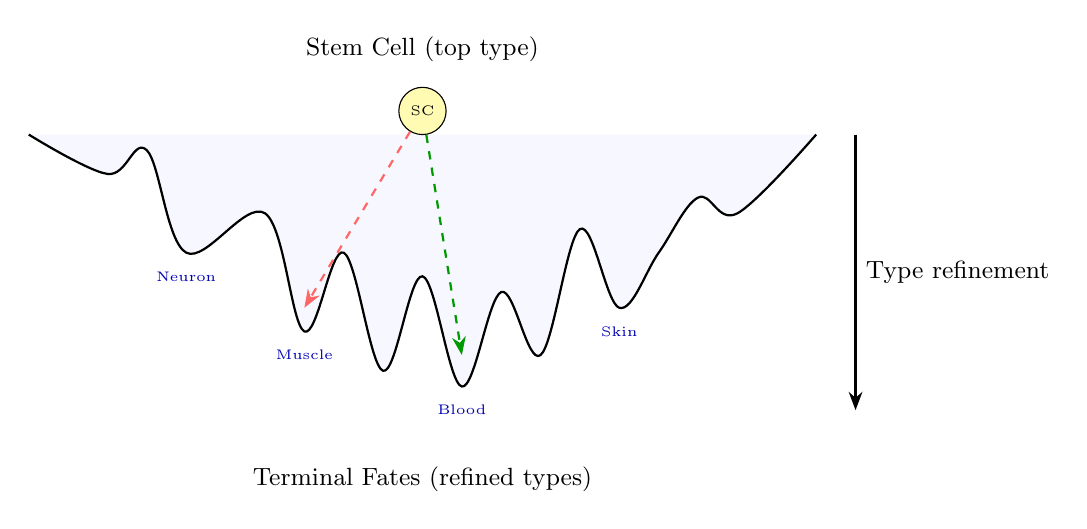
\begin{tikzpicture}[
  scale=1.0,
  cell/.style={circle, draw, fill=yellow!30, minimum size=6mm, inner sep=0pt, font=\tiny},
  valley/.style={draw, thick, fill=blue!5},
  >=Stealth
]
  % The landscape
  \draw[thick, fill=blue!3] plot[smooth, tension=0.6]
    coordinates {(-5,4) (-4,3.5) (-3.5,3.8) (-3,2.5) (-2,3) (-1.5,1.5)
    (-1,2.5) (-0.5, 1.0) (0,2.2) (0.5,0.8) (1,2.0) (1.5,1.2)
    (2,2.8) (2.5, 1.8) (3,2.5) (3.5,3.2) (4,3.0) (5,4)};

  % Valley labels
  \node[font=\tiny, text=blue!70!black] at (-3, 2.2) {Neuron};
  \node[font=\tiny, text=blue!70!black] at (-1.5, 1.2) {Muscle};
  \node[font=\tiny, text=blue!70!black] at (0.5, 0.5) {Blood};
  \node[font=\tiny, text=blue!70!black] at (2.5, 1.5) {Skin};

  % Ball (cell) at top
  \node[cell] (ball) at (0, 4.3) {SC};
  \draw[->, thick, red!60, dashed] (ball) -- (-1.5, 1.8);
  \draw[->, thick, green!60!black, dashed] (ball) -- (0.5, 1.2);

  % Labels
  \node[font=\small, above] at (0, 4.8) {Stem Cell (top type)};
  \node[font=\small, below] at (0, -0.1) {Terminal Fates (refined types)};

  % Refinement arrow
  \draw[->, thick] (5.5, 4) -- (5.5, 0.5) node[midway, right, font=\small] {Type refinement};
\end{tikzpicture}
\caption{The Waddington landscape as a refinement-type lattice.
  The stem cell (top type) rolls downhill through progressive refinement
  to terminal cell fates (maximally refined types).}
\label{fig:waddington}
\end{figure}

\begin{definition}[Refinement Path]\label{def:refinement-path}
A \emph{refinement path} through the Waddington landscape is a
sequence of types:
\[
  \StemCell = T_0 \sqsupseteq T_1 \sqsupseteq \cdots \sqsupseteq
  T_n = \TermCell
\]
where each $T_{i+1}$ is obtained from $T_i$ by responding to a
specific inductive signal $s_i$.  The path is \emph{deterministic}
given the signal sequence $(s_0, s_1, \ldots, s_{n-1})$.
\end{definition}


% ═══════════════════════════════════════════════════════════════
\section{Morphogen Gradient as Dependent Type}\label{sec:morphogen-dependent}
% ═══════════════════════════════════════════════════════════════

The French flag model (\cref{sec:morphogens}) assigns discrete cell fates
based on morphogen concentration.  We now formalize this as a
\emph{dependent type}: the cell-fate type \emph{depends on} the
cell's spatial position and the local morphogen concentration.

\begin{definition}[Spatially-Dependent Cell Fate]\label{def:dependent-fate}
Define the dependent type:
\[
  \texttt{CellFate} : \Omega \times \mathbb{R}_{\geq 0} \to \mathsf{Type}
\]
such that $\texttt{CellFate}(\mathbf{x}, c)$ is the cell type assigned
to a cell at position $\mathbf{x}$ experiencing morphogen concentration $c$.
\end{definition}

\begin{theorem}[Dependent Type Consistency]\label{thm:dependent-consistency}
For a well-formed morphogen field $(M, \Omega, c)$, the dependent
type $\texttt{CellFate}(\mathbf{x}, c(\mathbf{x},t))$ satisfies:
\begin{enumerate}
  \item \emph{Local consistency}: Nearby cells with similar
    concentrations receive compatible types.
    \[
      |\mathbf{x} - \mathbf{y}| < \epsilon \implies
      \texttt{CellFate}(\mathbf{x}, c(\mathbf{x},t)) =
      \texttt{CellFate}(\mathbf{y}, c(\mathbf{y},t))
    \]
    when $\mathbf{x}$ and $\mathbf{y}$ lie in the same French flag zone.
  \item \emph{Boundary sharpness}: At zone boundaries, the type
    assignment changes discretely despite continuous concentration.
  \item \emph{Temporal stability}: Once determined, the type
    assignment is maintained even if the morphogen field dissipates.
\end{enumerate}
\end{theorem}

\begin{proof}
(1) follows from the piecewise-constant nature of the French flag
partition.  (2) follows from threshold-based switching.  (3) follows
from the cell-autonomous maintenance of fate via auto-regulatory
transcription factor networks that lock in the determined state,
analogous to a latch in digital logic.
\end{proof}

The dependent-type perspective unifies several phenomena:

\begin{corollary}
The following are all instances of dependent typing:
\begin{enumerate}
  \item \textbf{Dorsal--ventral patterning}: $\texttt{CellFate}(y, [\text{BMP}](y))$
    where $y$ is the D--V coordinate.
  \item \textbf{Limb bud patterning}: $\texttt{CellFate}(x, y, z,
    [\text{Shh}](x), [\text{FGF}](y), [\text{Wnt}](z))$ with three
    morphogen axes.
  \item \textbf{Somitogenesis}: $\texttt{CellFate}(x, t, [\text{Notch}](x,t))$
    where the oscillatory Notch signal creates periodic segments.
\end{enumerate}
\end{corollary}


% ═══════════════════════════════════════════════════════════════
\section{Hox Collinearity as Monotone Functor}\label{sec:hox-functor}
% ═══════════════════════════════════════════════════════════════

We now formalize the collinearity property of Hox genes in
category-theoretic terms.

\begin{definition}[Ordered Sets as Categories]\label{def:ordered-cat}
An ordered set $(S, \leq)$ can be viewed as a thin category
$\mathbf{S}$ where:
\begin{itemize}
  \item Objects are elements of $S$.
  \item There is a unique morphism $s_1 \to s_2$ iff $s_1 \leq s_2$.
\end{itemize}
\end{definition}

\begin{definition}[Chromosome and Body-Axis Categories]\label{def:chr-body-cat}
Define:
\begin{itemize}
  \item $\mathbf{Chr} = (\{1, 2, \ldots, n\}, \leq)$: the category
    of chromosomal positions of Hox genes.
  \item $\mathbf{Axis} = (\{A, \ldots, P\}, \leq_{AP})$: the category
    of anterior--posterior body positions.
\end{itemize}
\end{definition}

\begin{theorem}[Collinearity Functor]\label{thm:collinearity-functor}
Hox spatial collinearity is a \emph{monotone functor}
$F : \mathbf{Chr} \to \mathbf{Axis}$ satisfying:
\begin{enumerate}
  \item $F$ maps each chromosomal position to a body-axis position.
  \item $F$ preserves order: if $i \leq_{\text{chr}} j$, then
    $F(i) \leq_{AP} F(j)$.
\end{enumerate}
Similarly, temporal collinearity is a monotone functor
$G : \mathbf{Chr} \to \mathbf{Time}$ where $\mathbf{Time} =
(\mathbb{R}_{\geq 0}, \leq)$.
\end{theorem}

\begin{proof}
The functor $F$ is defined by the spatial expression function
$\sigma$ from \cref{def:hox-cluster}: $F(i) = \max(\sigma(H_i))$.
By \cref{ax:spatial-col}, $i \leq_{\text{chr}} j$ implies
$F(i) \leq_{AP} F(j)$, so $F$ preserves order and is thus a
monotone functor.  The argument for $G$ using $\tau$ and
\cref{ax:temporal-col} is identical.
\end{proof}

\begin{corollary}[Collinearity as Natural Transformation]
When both spatial and temporal collinearity hold, the pair
$(F, G)$ constitutes a \emph{joint monotone functor}
$\mathbf{Chr} \to \mathbf{Axis} \times \mathbf{Time}$,
expressing the fact that chromosomal order simultaneously
determines both spatial and temporal expression patterns.
\end{corollary}

\[
\begin{tikzcd}
  \mathbf{Chr} \arrow[r, "F"] \arrow[dr, "G"'] &
    \mathbf{Axis} \\
  & \mathbf{Time}
\end{tikzcd}
\qquad\Longrightarrow\qquad
\begin{tikzcd}
  \mathbf{Chr} \arrow[r, "{(F,G)}"] & \mathbf{Axis} \times \mathbf{Time}
\end{tikzcd}
\]


% ═══════════════════════════════════════════════════════════════
\section{Organogenesis as Container Orchestration}\label{sec:organogenesis}
% ═══════════════════════════════════════════════════════════════

Organogenesis---the formation of organs from groups of cells---bears
a remarkable structural similarity to container orchestration in
modern distributed systems.  We develop this analogy formally.

\begin{definition}[Tissue as Container]\label{def:tissue-container}
A \emph{tissue container} is a tuple $T = (C, I, R, H)$ where:
\begin{itemize}
  \item $C \subset \texttt{Cell}$ is the set of cells in the tissue.
  \item $I : C \to \mathsf{CellType}$ is the cell-type assignment
    (the ``image'' each cell runs).
  \item $R : C \to \text{Resources}$ specifies resource requirements
    (nutrients, oxygen, growth factors).
  \item $H : C \to \{0,1\}$ is the health check function.
\end{itemize}
\end{definition}

\begin{definition}[Organ as Pod]\label{def:organ-pod}
An \emph{organ pod} is a collection of tissue containers that
cooperate to provide a physiological function:
\[
  O = \{T_1, T_2, \ldots, T_k\}
\]
equipped with:
\begin{itemize}
  \item \emph{Inter-tissue signaling}: Communication channels
    between tissues (paracrine signaling $\approx$ inter-container
    networking).
  \item \emph{Shared resources}: Common extracellular matrix and
    vasculature ($\approx$ shared volumes).
  \item \emph{Specification}: A declarative description of the
    organ's target state ($\approx$ deployment manifest).
\end{itemize}
\end{definition}

\begin{table}[H]
\centering
\begin{tabular}{ll}
\toprule
\textbf{Container Orchestration} & \textbf{Organogenesis} \\
\midrule
Container & Cell \\
Pod & Organ primordium \\
Service & Tissue type \\
Deployment manifest & Developmental gene network \\
Scheduler & Morphogen gradient \\
Health check & Cell viability signaling \\
Auto-scaling & Compensatory proliferation \\
Rolling update & Tissue remodeling \\
Namespace & Germ layer (ectoderm/mesoderm/endoderm) \\
ConfigMap & Morphogen concentration profile \\
Secret & Intracellular signaling state \\
\bottomrule
\end{tabular}
\caption{Container orchestration $\leftrightarrow$ organogenesis correspondence.}
\label{tab:orchestration}
\end{table}

\begin{theorem}[Organ Assembly as Typed Orchestration]\label{thm:organ-orch}
Organ assembly can be modeled as a typed orchestration program where:
\begin{enumerate}
  \item Each tissue container has a typed interface specifying its
    signaling inputs and outputs.
  \item Container composition is type-checked: tissues can only
    be assembled if their interfaces are compatible.
  \item The orchestrator (morphogen fields + regulatory networks)
    ensures that tissue containers are deployed in the correct
    spatial arrangement and temporal order.
\end{enumerate}
\end{theorem}

\begin{proof}
The interface of a tissue container $T_i$ is the pair
$(\text{In}_i, \text{Out}_i)$ of required input signals and
provided output signals.  Compatibility requires that for each
required input of $T_i$, there exists another container $T_j$
in the organ pod whose output provides that signal.  This is
precisely interface compatibility checking in a typed module system.
The morphogen field provides the spatial scheduling information
(which containers go where), and the regulatory network provides
temporal ordering (which containers start first).
\end{proof}

\begin{example}[Kidney Organogenesis]
Kidney development illustrates container orchestration:
\begin{enumerate}
  \item \textbf{Ureteric bud} (container 1): Expresses Ret receptor,
    branches iteratively.
  \item \textbf{Metanephric mesenchyme} (container 2): Expresses GDNF
    (signals to ureteric bud), receives Wnt signals.
  \item \textbf{Signaling interface}: GDNF (mesenchyme $\to$ bud),
    Wnt9b (bud $\to$ mesenchyme).
  \item \textbf{Orchestration}: Reciprocal induction creates a
    feedback loop that drives iterative branching and nephron formation.
\end{enumerate}
\end{example}


% ═══════════════════════════════════════════════════════════════
\section{Haskell Implementation}\label{sec:implementation}
% ═══════════════════════════════════════════════════════════════

We provide a complete Haskell implementation that demonstrates the
key abstractions of our framework.  The implementation compiles with
GHC and uses no external dependencies.

\subsection{Module Structure}

The implementation is organized into five modules:

\begin{itemize}[leftmargin=2em]
  \item \texttt{Program.hs}: Core \texttt{Program} type and
    developmental stage transitions.
  \item \texttt{BodyPlan.hs}: Hox gene cluster, collinearity
    mapping, segment identity.
  \item \texttt{RegulatoryNetwork.hs}: Master regulator cascades,
    feed-forward loops, regulatory graph traversal.
  \item \texttt{Differentiation.hs}: Waddington landscape, cell
    fate decisions, stem cell $\to$ terminal cell paths, apoptosis.
  \item \texttt{Main.hs}: Demonstration of all components.
\end{itemize}

\subsection{Core Program Type}

\begin{lstlisting}
data DevStage = Cleavage | Gastrulation | Organogenesis | Maturation
  deriving (Show, Eq, Ord, Enum, Bounded)

data Program d = Program
  { hoxCluster       :: HoxCluster
  , morphogens       :: [MorphogenField]
  , cellPopulation   :: [Cell]
  , regulatoryNet    :: RegNetwork
  , signalingState   :: SignalState
  , developmental_stage :: d
  }
\end{lstlisting}

\subsection{Hox Collinearity Verification}

\begin{lstlisting}
verifyCollinearity :: HoxCluster -> Bool
verifyCollinearity cluster =
  let genes = hoxGenes cluster
      positions = map chromosomePosition genes
      bodyPositions = map (axisPosition . expressionDomain) genes
  in isSorted positions && isSorted bodyPositions
  where
    isSorted [] = True
    isSorted [_] = True
    isSorted (x:y:xs) = x <= y && isSorted (y:xs)
\end{lstlisting}

\subsection{Morphogen Gradient Interpretation}

\begin{lstlisting}
interpretGradient :: MorphogenField -> Double -> CellFateZone
interpretGradient field concentration
  | concentration > highThreshold field = HighZone
  | concentration > midThreshold field  = MidZone
  | concentration > lowThreshold field  = LowZone
  | otherwise                           = NoSignal
\end{lstlisting}

\subsection{Cell Fate Decision Tree}

\begin{lstlisting}
decideFate :: Cell -> [Signal] -> Cell
decideFate cell signals = case cellState cell of
  Stem potency -> case findSignal signals InductiveSignal of
    Just sig -> specifyCell cell sig
    Nothing  -> maintainStemness cell
  Progenitor lineage -> case findSignal signals DetermSignal of
    Just sig -> determineCell cell sig
    Nothing  -> cell
  Determined fate -> case findSignal signals DiffSignal of
    Just _ -> differentiate cell
    Nothing -> cell
  Terminal _ -> cell  -- already fully differentiated
\end{lstlisting}

\subsection{Waddington Landscape Simulation}

\begin{lstlisting}
simulateWaddington :: Cell -> [Signal] -> [Cell]
simulateWaddington cell [] = [cell]
simulateWaddington cell (s:ss) =
  let cell' = decideFate cell [s]
  in cell : simulateWaddington cell' ss
\end{lstlisting}

\subsection{Regulatory Boot Sequence}

\begin{lstlisting}
bootSequence :: RegNetwork -> [TFActivation]
bootSequence network =
  topologicalSort (regNodes network) (regEdges network)
\end{lstlisting}

The full implementation, including all type definitions, helper
functions, and demonstration code, is provided in the accompanying
source files.


% ═══════════════════════════════════════════════════════════════
\section{Discussion and Conclusion}\label{sec:discussion}
% ═══════════════════════════════════════════════════════════════

\subsection{Synthesis}

This paper has established a comprehensive type-theoretic framework
for developmental biology.  The key insight is that the developmental
program of a multicellular organism is not merely \emph{analogous to}
a computer program---it \emph{is} a program in a precise technical
sense, with types, modules, dependencies, and execution semantics
that map faithfully onto constructs from programming-language theory.

\begin{table}[H]
\centering
\begin{tabular}{ll}
\toprule
\textbf{Biological Concept} & \textbf{Type-Theoretic Formalization} \\
\midrule
Hox gene cluster & Main module \\
Morphogen gradient & Dependent type / distributed config \\
Cell-fate determination & Refinement-type narrowing \\
Waddington landscape & Refinement-type lattice \\
Regulatory cascade & Typed boot sequence (DAG) \\
Apoptosis & Linear-type resource consumption \\
Stem cell & Abstract factory with polymorphic constructors \\
Hox collinearity & Monotone functor \\
Organogenesis & Container orchestration \\
Developmental stage & Phantom type parameter \\
Homeotic mutation & Type error in main module \\
Cancer & Type-safety violation \\
\bottomrule
\end{tabular}
\caption{Complete correspondence between developmental biology and type theory.}
\label{tab:correspondence}
\end{table}

\subsection{The DNA-Lang Project: A Retrospective}

This paper concludes the seven-paper DNA-Lang project, which has
progressively developed a type-theoretic interpretation of the
genome:

\begin{enumerate}
  \item \textbf{Paper 1}: Coding sequences as executable functions.
  \item \textbf{Paper 2}: Regulatory sequences as control flow.
  \item \textbf{Paper 3}: Noncoding RNA as type-level metaprogramming.
  \item \textbf{Paper 4}: Epigenetic marks as compiler pragmas.
  \item \textbf{Paper 5}: Repetitive elements as memory architecture.
  \item \textbf{Paper 6}: Structural DNA as runtime environment.
  \item \textbf{Paper 7}: Developmental programs as orchestration
    (this paper).
\end{enumerate}

Together, these papers establish that the genome is not merely a
passive database of gene sequences but an \emph{active programming
language} with a rich type system, modular architecture, and
sophisticated execution semantics.

\subsection{Implications for Biology}

The type-theoretic framework offers several concrete benefits for
biological reasoning:

\begin{enumerate}[leftmargin=2em]
  \item \textbf{Prediction}: Type-checking developmental programs
    can predict which mutations will be lethal (type errors in
    essential modules), which will produce homeotic transformations
    (type errors in the Hox main module), and which will be tolerated
    (changes within a type's implementation that preserve its interface).
  \item \textbf{Disease understanding}: Cancer is a type-safety
    violation where cells escape their refinement constraints.
    Developmental disorders are compile-time errors.  Aging is
    type erosion from accumulated runtime errors.
  \item \textbf{Synthetic biology}: Engineering organisms becomes
    a programming task with type guidance.  Well-typed developmental
    programs should produce well-formed organisms.
\end{enumerate}

\subsection{Implications for Computer Science}

Biology, in turn, offers lessons for programming-language design:

\begin{enumerate}[leftmargin=2em]
  \item \textbf{Robustness}: Developmental programs are extraordinarily
    robust to perturbation, suggesting that biological type systems
    have sophisticated error-correction mechanisms we have yet to
    replicate.
  \item \textbf{Self-organization}: Morphogen-based configuration is
    inherently decentralized, suggesting alternatives to centralized
    orchestration systems.
  \item \textbf{Graceful degradation}: Apoptosis and compensatory
    proliferation suggest that programs should be designed to lose
    components gracefully.
\end{enumerate}

\subsection{Limitations and Future Work}

Our framework currently treats development as a deterministic,
well-typed process.  In reality, stochastic gene expression,
environmental perturbation, and epigenetic noise introduce
non-determinism.  Future work should incorporate:

\begin{itemize}[leftmargin=2em]
  \item \emph{Probabilistic types} to model stochastic fate decisions.
  \item \emph{Gradual typing} to model the spectrum from labile
    specification to irreversible determination.
  \item \emph{Session types} to model the dynamic signaling
    conversations between cells during induction.
  \item \emph{Spatial type systems} that natively encode the
    three-dimensional geometry of developing tissues.
\end{itemize}

\subsection{Conclusion}

From genome to organism, development is orchestration.  The DNA-Lang
project has shown that this is not merely a metaphor but a formal
correspondence, with each biological mechanism mapping to a precise
type-theoretic construct.  The genome is a program; the cell is a
runtime; and the organism is the well-typed output of a developmental
orchestration engine that has been refined by four billion years of
evolution.

\bigskip

\noindent\textbf{Acknowledgments.}
The author thanks the YonedaAI Collaboration for ongoing support
and the broader communities at the intersection of biology, category
theory, and programming-language theory.

% ─── References ────────────────────────────────────────────────
\begin{thebibliography}{99}

\bibitem{waddington1957}
C.~H. Waddington.
\newblock \emph{The Strategy of the Genes}.
\newblock George Allen \& Unwin, London, 1957.

\bibitem{wolpert1969}
L.~Wolpert.
\newblock Positional information and the spatial pattern of cellular
  differentiation.
\newblock \emph{Journal of Theoretical Biology}, 25(1):1--47, 1969.

\bibitem{mcginnis1992}
W.~McGinnis and R.~Krumlauf.
\newblock Homeobox genes and axial patterning.
\newblock \emph{Cell}, 68(2):283--302, 1992.

\bibitem{duboule2007}
D.~Duboule.
\newblock The rise and fall of Hox gene clusters.
\newblock \emph{Development}, 134(14):2549--2560, 2007.

\bibitem{turing1952}
A.~M. Turing.
\newblock The chemical basis of morphogenesis.
\newblock \emph{Philosophical Transactions of the Royal Society B},
  237(641):37--72, 1952.

\bibitem{martinlof1984}
P.~Martin-L\"of.
\newblock \emph{Intuitionistic Type Theory}.
\newblock Bibliopolis, Naples, 1984.

\bibitem{wadler2015}
P.~Wadler.
\newblock Propositions as types.
\newblock \emph{Communications of the ACM}, 58(12):75--84, 2015.

\bibitem{pierce2002}
B.~C. Pierce.
\newblock \emph{Types and Programming Languages}.
\newblock MIT Press, Cambridge, MA, 2002.

\bibitem{girard1987}
J.-Y. Girard.
\newblock Linear logic.
\newblock \emph{Theoretical Computer Science}, 50(1):1--102, 1987.

\bibitem{huang2005}
S.~Huang.
\newblock Reprogramming cell fates: reconciling rarity with
  robustness.
\newblock \emph{BioEssays}, 31(5):546--560, 2009.

\bibitem{keller2005}
R.~Keller.
\newblock Cell migration during gastrulation.
\newblock \emph{Current Opinion in Cell Biology}, 17(5):533--541, 2005.

\bibitem{green2015}
J.~B.~A. Green and J.~Sharpe.
\newblock Positional information and reaction-diffusion: two big ideas
  in developmental biology combine.
\newblock \emph{Development}, 142(7):1203--1211, 2015.

\bibitem{elowitz2002}
M.~B. Elowitz and S.~Leibler.
\newblock A synthetic oscillatory network of transcriptional regulators.
\newblock \emph{Nature}, 403(6767):335--338, 2000.

\bibitem{burns2005}
K.~Burns et al.
\newblock Container-based operating system virtualization.
\newblock \emph{Proceedings of EuroSys}, 2016.

\bibitem{freeman2002}
M.~Freeman.
\newblock Feedback control of intercellular signalling in development.
\newblock \emph{Nature}, 408(6810):313--319, 2000.

\bibitem{takahashi2006}
K.~Takahashi and S.~Yamanaka.
\newblock Induction of pluripotent stem cells from mouse embryonic and
  adult fibroblast cultures by defined factors.
\newblock \emph{Cell}, 126(4):663--676, 2006.

\end{thebibliography}

\end{document}
